\documentclass[11pt,letterpaper]{article}
\usepackage{scientific_report}
\usepackage{pgfplots}
\pgfplotsset{compat=1.18}
\usepackage{float}
\usepackage{listings}
\usepackage{xcolor}
\usepackage{geometry}
\geometry{headheight=23pt, top=2cm, bottom=2cm, left=2.5cm, right=2.5cm}
\setlength{\parskip}{0.5em}
\setlength{\parindent}{0pt}

\lstset{
    language=C,
    basicstyle=\ttfamily\small,
    keywordstyle=\color{blue}\bfseries,
    commentstyle=\color{green!60!black}\itshape,
    stringstyle=\color{red!80!black},
    numbers=left,
    numberstyle=\tiny\color{gray},
    numbersep=8pt,
    frame=single,
    breaklines=true,
    captionpos=b,
    tabsize=4,
    showstringspaces=false
}

\begin{document}
\pagestyle{plain}

\begin{center}
    {\LARGE\bfseries Aproximação de $\pi$ usando Série Matemática}\\[0.5em]
    {\large Análise de Precisão e Desempenho Computacional}\\[1em]
    {\normalsize Eugênio Vitor Lopes dos Santos}\\[0.3em]
    {\small DCA3703 - Programação Paralela --- Universidade Federal do Rio Grande do Norte}\\[0.3em]
    {\small 2026}
\end{center}

\vspace{1em}

\section{Enunciado}

Implemente um programa em C que calcule uma aproximação de $\pi$ usando uma série matemática, variando o número de iterações e medindo o tempo de execução. Compare os valores obtidos com o valor real de $\pi$ e analise como a acurácia melhora com mais processamento. Reflita sobre como esse comportamento se repete em aplicações reais que demandam resultados cada vez mais precisos, como simulações físicas e inteligência artificial.

% 2. Fundamentação Teórica
\section{Fundamentação Teórica}

\subsection{Série de Leibniz}
A série de Leibniz para $\pi$ é dada por:
\[
\pi = 4 \sum_{k=0}^{\infty} \frac{(-1)^k}{2k+1} = 4 \left(1 - \frac{1}{3} + \frac{1}{5} - \frac{1}{7} + \frac{1}{9} - \cdots\right)
\]


\subsection{Algoritmo}
\begin{enumerate}
    \item Inicializar \texttt{pi} = 0.0
    \item Para cada iteração $k$ de 0 até $N-1$:
    \begin{itemize}
        \item Calcular termo: $\frac{1}{2k+1}$
        \item Aplicar sinal alternado: positivo para $k$ par, negativo para $k$ ímpar
        \item Acumular o termo
    \end{itemize}
    \item Multiplicar o resultado por 4
    \item Calcular o erro absoluto: $|\pi_{aprox} - \pi_{real}|$
\end{enumerate}

% 3. Experimento
\newpage
\section{Experimento}

\subsection{Código-Fonte}
O programa recebe o número de iterações como argumento de linha de comandos e calcula a aproximação de $\pi$ pela série de Leibniz.

\begin{lstlisting}[caption={Código-fonte em C para Aproximação de $\pi$}, label={lst:codigo}]
#include <stdio.h>
#include <stdlib.h>
#include <math.h>

int main(int argc, char *argv[]) {
    if (argc != 2) {
        printf("Uso: %s <numero_de_iteracoes>\n", argv[0]);
        return 1;
    }

    long long N = atoll(argv[1]);
    double pi = 0.0;

    for (long long k = 0; k < N; k++) {
        double termo = 1.0 / (2.0 * k + 1.0);
        pi += (k % 2 == 0) ? termo : -termo;
    }
    pi *= 4.0;

    double erro = fabs(pi - M_PI);

    printf("Iteracoes: %lld\n", N);
    printf("Pi:        %.15f\n", pi);
    printf("Erro:      %.2e\n", erro);

    return 0;
}
\end{lstlisting}

O tempo de execução é medido externamente com o comando \texttt{time} do shell Linux, variando o argumento de iterações a cada execução:
\begin{lstlisting}[caption={Exemplo de execução com medição de tempo}, label={lst:execucao}]
gcc tarefa01.c -o tarefa01 -lm
time ./tarefa01 1000000000
\end{lstlisting}

% 4. Resultados
\newpage
\section{Resultados}

\subsection{Dados Coletados}

\begin{table}[H]
\centering
\caption{Resultados da Aproximação de $\pi$}
\label{tab:results}
\small
\begin{tabular}{@{}lccc@{}}
\toprule
\textbf{Iterações} & \textbf{$\pi$ Aproximado} & \textbf{Erro Absoluto} & \textbf{Tempo (s)} \\
\midrule
1 & 4.000000000000000 & 8.58e-01 & 0.002 \\
10 & 3.041839618929403 & 9.98e-02 & 0.001 \\
100 & 3.131592903558554 & 1.00e-02 & 0.002 \\
1.000 & 3.140592653839794 & 1.00e-03 & 0.002 \\
10.000 & 3.141492653590034 & 1.00e-04 & 0.002 \\
100.000 & 3.141582653589720 & 1.00e-05 & 0.002 \\
1.000.000 & 3.141591653589774 & 1.00e-06 & 0.004 \\
10.000.000 & 3.141592553589792 & 1.00e-07 & 0.022 \\
100.000.000 & 3.141592643589326 & 1.00e-08 & 0.240 \\
1.000.000.000 & 3.141592652588050 & 1.00e-09 & 1.943 \\
10.000.000.000 & 3.141592653488346 & 1.01e-10 & 17.408 \\
100.000.000.000 & 3.141592653578537 & 1.13e-11 & 188.135 \\
\bottomrule
\end{tabular}
\end{table}

\subsection{Análise Visual}

\begin{figure}[H]
\centering
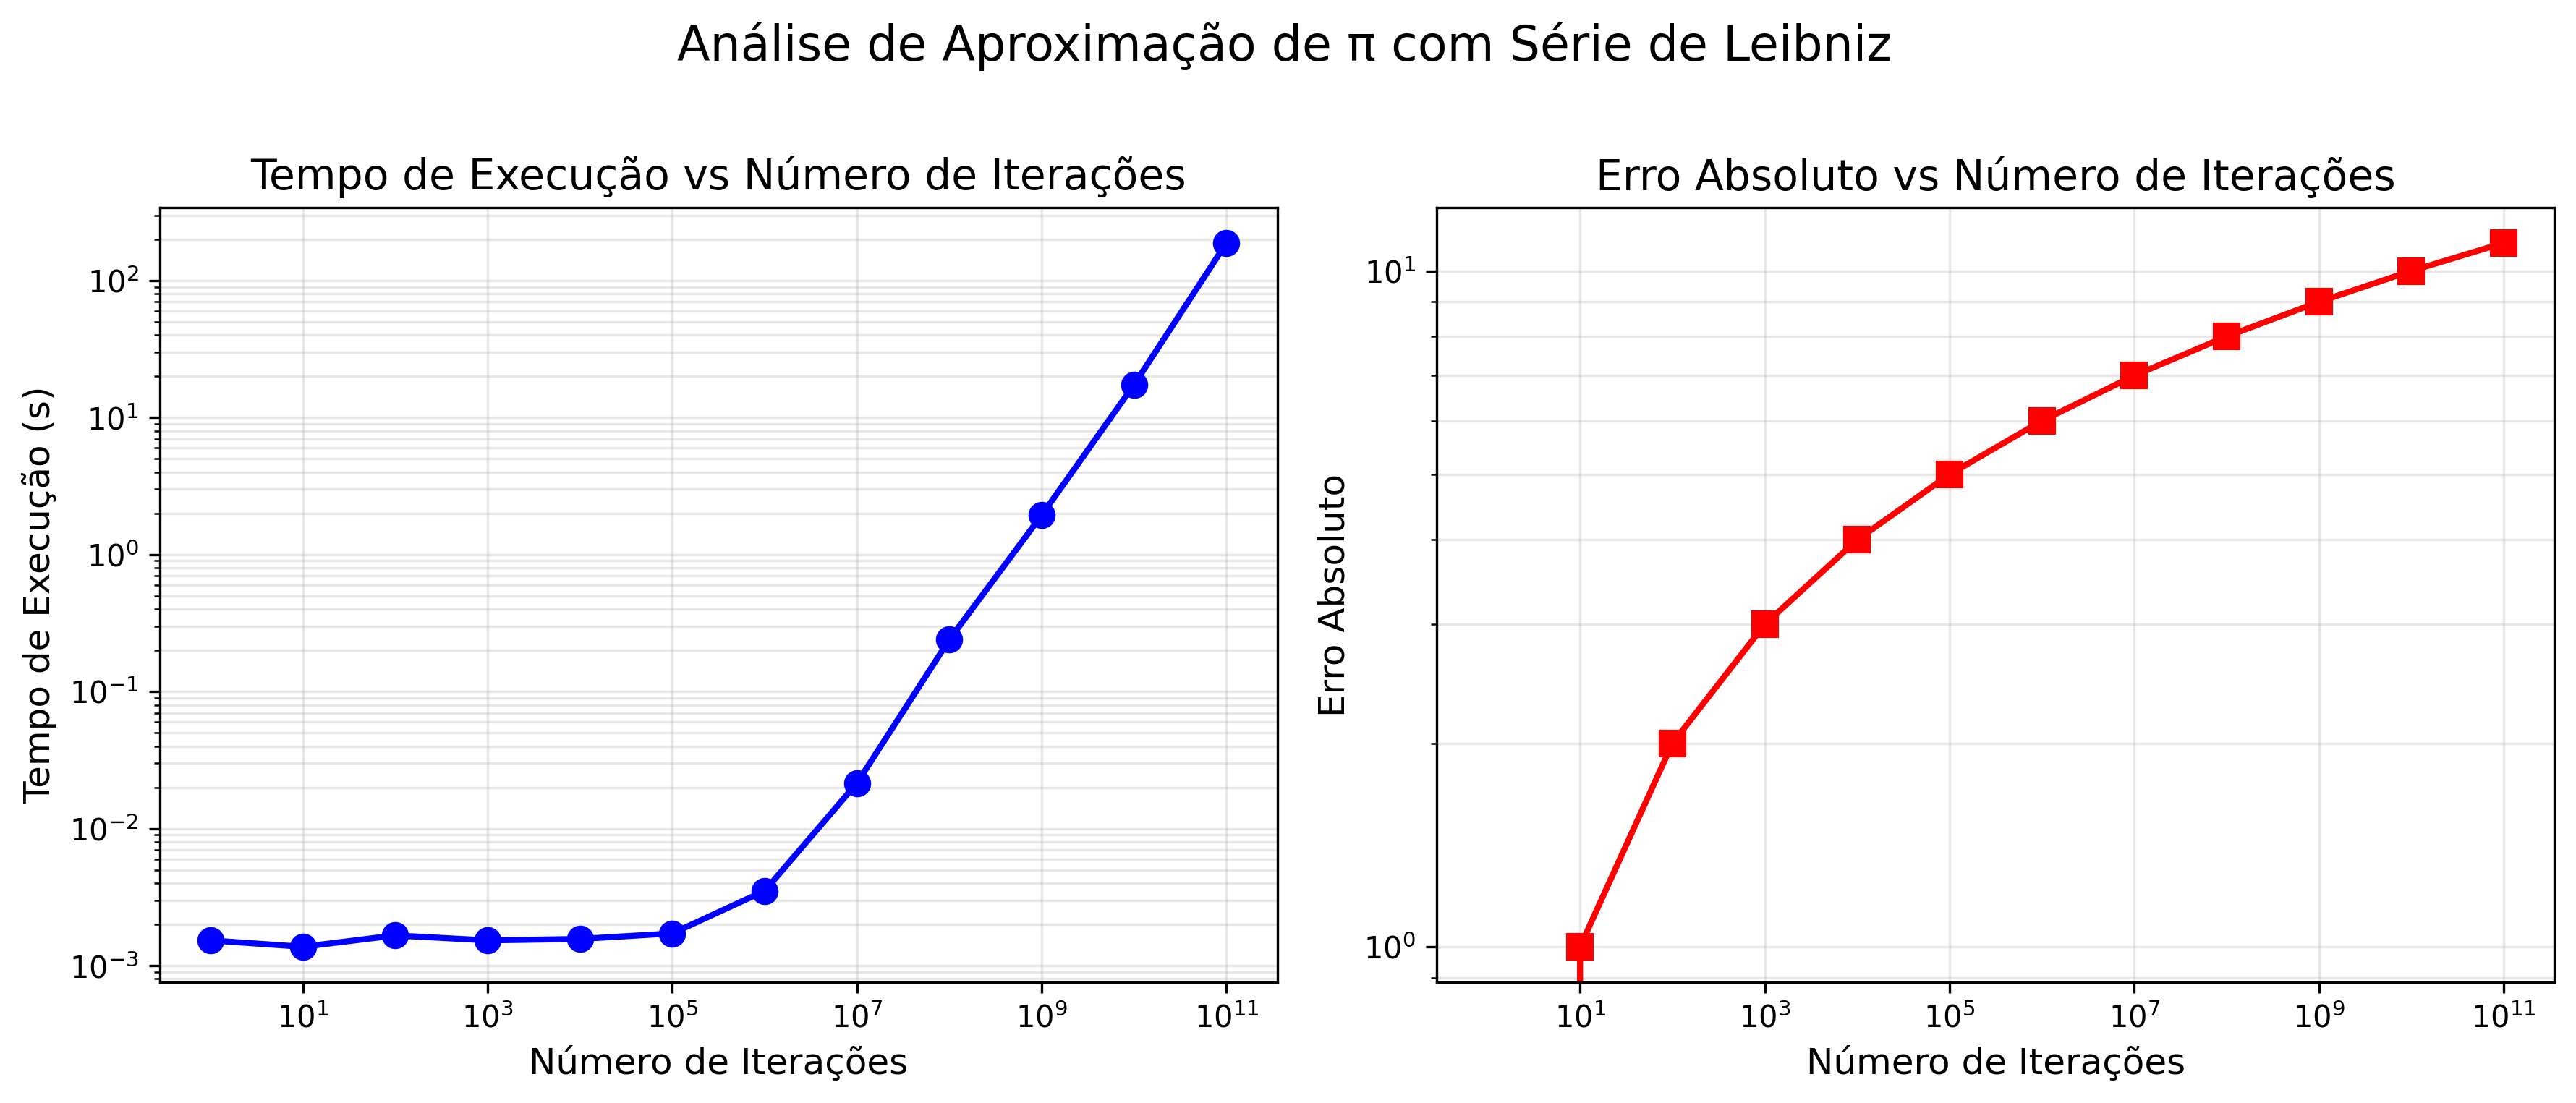
\includegraphics[width=0.9\textwidth]{pi_approximation_analysis.png}
\caption{Análise da Aproximação de $\pi$: (a) Tempo de Execução vs Iterações; (b) Erro Absoluto vs Iterações. Ambos os eixos em escala logarítmica.}
\label{fig:analysis}
\end{figure}

\subsection{Observações Principais}
\begin{itemize}
    \item O erro absoluto diminui uma ordem de magnitude a cada 10x mais iterações.
    \item O tempo de execução cresce linearmente com o número de iterações.
    \item A precisão de $10^{-9}$ foi alcançada com 1 bilhão de iterações.
\end{itemize}

% 5. Discussão
\section{Discussão}

Esse trade-off entre precisão e custo computacional é justamente o que motiva o uso de técnicas de paralelização e séries de convergência mais rápida. Séries alternativas a Leibniz, como a série de Machin ou algoritmos como o de Chudnovsky, convergem muito mais rapidamente, exigindo menos iterações para o mesmo nível de precisão. Da mesma forma, distribuir o cálculo entre múltiplos núcleos ou GPUs permite reduzir o tempo de execução sem abrir mão da precisão desejada, abordagem central em simulações físicas de larga escala e no treinamento de modelos de IA modernos, que dependem intensamente de paralelismo (múltiplas CPUs/GPUs) para tornar viável o processamento de dados em escala.

\section{Conclusão}
O experimento demonstra, em escala reduzida, um princípio fundamental da computação científica: precisão tem custo computacional, e esse custo cresce de forma desproporcional ao ganho de precisão obtido. Esse mesmo princípio orienta decisões de engenharia em áreas muito mais complexas, como simulações físicas e inteligência artificial, onde a escolha entre algoritmos mais eficientes, paralelização e trade-offs de precisão é frequentemente o que determina a viabilidade prática de um projeto.

\end{document}
